\documentclass[12pt,a4paper]{article}
\usepackage{fontspec}
%L2W-FONT-BEGIN (bộ kiểm thử thay khối này bằng tệp phông có thật trên máy khi biên dịch)
\IfFontExistsTF{TeX Gyre Termes}{\setmainfont{TeX Gyre Termes}}{%
  \IfFontExistsTF{Times New Roman}{\setmainfont{Times New Roman}}{}}
%L2W-FONT-END
\usepackage{amsmath,amssymb}
\usepackage{tikz,tkz-tab}
\usepackage[margin=2cm]{geometry}
\newcommand{\vecto}[1]{\overrightarrow{#1}}
\begin{document}
\section*{Đề kiểm tra mẫu}

\textbf{Câu 1.} Cho hàm số $y=x^3-3x+1$. Giá trị của biểu thức $\dfrac{a+1}{2}$ khi $a=3$ là

\noindent A. $1$.\hfill B. $2$.\hfill C. $3$.\hfill D. $4$.

\textbf{Câu 2.} Trong không gian, cho $\vecto{AB}=(1;2;3)$ và $\sqrt{x+1}=2$. Mệnh đề nào đúng?

\noindent A. Điểm $M$ thuộc đường thẳng $d$.\hfill B. Điểm $N$ không thuộc $d$.

\noindent C. Hai đường thẳng song song.\hfill D. Hai đường thẳng cắt nhau.

\textbf{Câu 3.} Tính tích phân sau:
\begin{equation}
\int_0^1 x^2\,dx=\frac{1}{3}.
\end{equation}

\textbf{Câu 4.} Bảng tần số ghép nhóm:
\begin{center}
\begin{tabular}{|c|c|c|c|}
\hline
Nhóm & $[0;5)$ & $[5;10)$ & $[10;15)$ \\ \hline
Tần số & 3 & 5 & 7 \\ \hline
\end{tabular}
\end{center}

\textbf{Câu 5.} Cho hàm số có bảng biến thiên:
\begin{center}
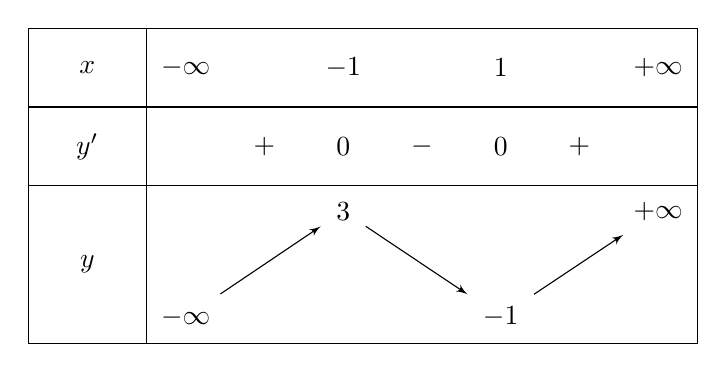
\begin{tikzpicture}
\tkzTabInit[lgt=1.5,espcl=2]{$x$/1,$y'$/1,$y$/2}{$-\infty$,$-1$,$1$,$+\infty$}
\tkzTabLine{,+,0,-,0,+,}
\tkzTabVar{-/$-\infty$,+/$3$,-/$-1$,+/$+\infty$}
\end{tikzpicture}
\end{center}

\noindent\begin{minipage}{0.6\textwidth}
\textbf{Câu 6.} Cho tam giác $ABC$ vuông tại $A$ như hình bên. Biết $AB=3$, $AC=4$. Tính độ dài cạnh $BC$.
\end{minipage}\hfill
\begin{minipage}{0.35\textwidth}
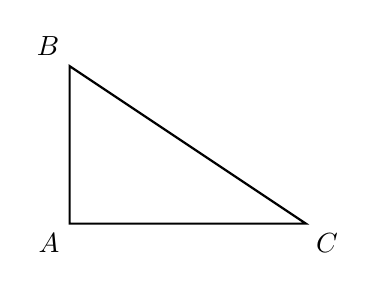
\begin{tikzpicture}
\draw[thick] (0,0) node[below left]{$A$} -- (3,0) node[below right]{$C$} -- (0,2) node[above left]{$B$} -- cycle;
\end{tikzpicture}
\end{minipage}

\end{document}
